\documentclass[11pt,a4paper]{article}
\usepackage[margin=2.2cm]{geometry}
\usepackage{graphicx,booktabs,amsmath,siunitx,xcolor,tabularx,enumitem}
\usepackage[version=4]{mhchem}
\usepackage[most]{tcolorbox}
\usepackage[hidelinks]{hyperref}
\graphicspath{{figures/}}
\setlist{itemsep=2pt,topsep=4pt}

% ---- note boxes -------------------------------------------------------------
\newtcolorbox{takeaway}{colback=blue!4,colframe=blue!50!black,boxrule=0.6pt,
  arc=2pt,left=6pt,right=6pt,top=4pt,bottom=4pt,fonttitle=\bfseries,title=Takeaway}
\newtcolorbox{pitfall}{colback=red!4,colframe=red!55!black,boxrule=0.6pt,
  arc=2pt,left=6pt,right=6pt,top=4pt,bottom=4pt,fonttitle=\bfseries,title=Pitfall}
\newtcolorbox{howto}{colback=gray!6,colframe=gray!60!black,boxrule=0.6pt,
  arc=2pt,left=6pt,right=6pt,top=4pt,bottom=4pt,fonttitle=\bfseries,title=How I did it}

\title{Study notes: visualising molecules for photocatalyst DFT}
\author{Lindejiade}
\date{October 2026 --- photocatalyst-dft project, week 1}

\begin{document}
\maketitle

\noindent The main thing I learned: \textbf{a molecular picture is a measurement tool, not decoration.}
Each kind of picture answers one question. A picture without a number next to it can
mislead, because what you see depends on choices (viewing angle, isovalue, colour scale) that
the molecule doesn't care about.

\begin{table}[h]
\centering
\begin{tabularx}{\linewidth}{@{}lllX@{}}
\toprule
Level & Tool & Input & Question it answers \\
\midrule
2D structure & RDKit & SMILES (graph only) & Is this the molecule and charge state I meant? \\
3D geometry & py3Dmol / RDKit & xyz coordinates & Is the shape sensible? Planar, twisted, crowded? \\
Before vs after & overlay & two xyz files & How far did DFT move the force-field structure? \\
Orbitals & PySCF $\to$ cube $\to$ viewer & MO coefficients & Where does the electron leave from and go to? \\
\bottomrule
\end{tabularx}
\end{table}

%=============================================================================
\section{2D depictions: checking the input}

A 2D drawing is computed from the bond graph alone, with no coordinates. It is the cheapest
check in the whole workflow, and it catches the most expensive mistakes: a missing bromine, a
neutral molecule that should be an ion, the wrong tautomer. These cost hours of DFT if they
reach the next step.

\begin{figure}[h]
\centering
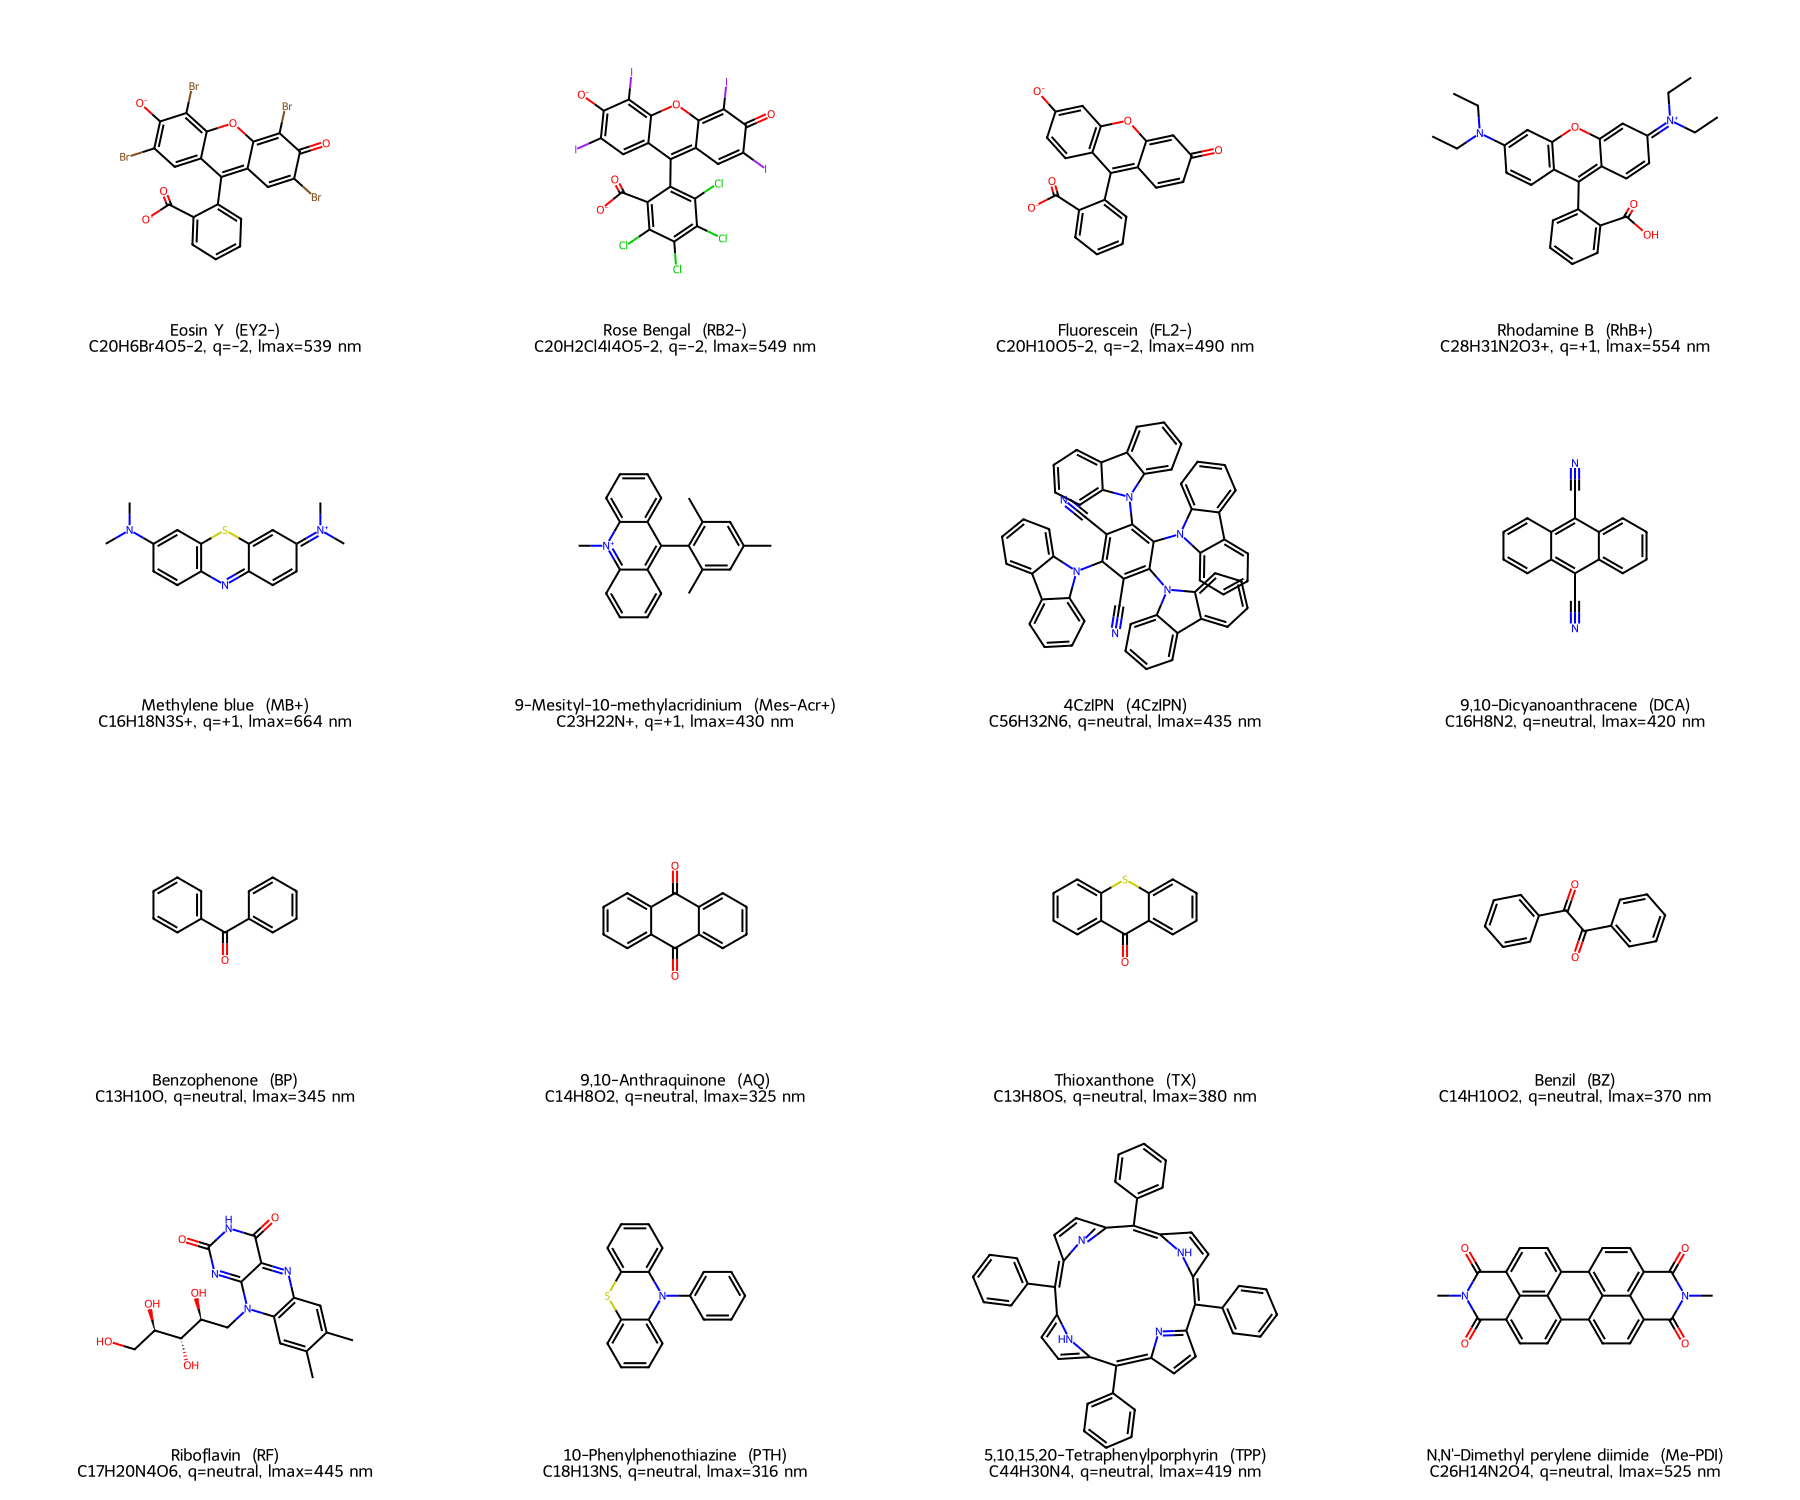
\includegraphics[width=0.92\linewidth]{organic_photocatalysts_grid.png}
\caption{The 16 organic photocatalysts as encoded. The first thing to look at is the charges:
\ce{EY^{2-}}, \ce{RB^{2-}} and \ce{FL^{2-}} are dianions, and \ce{MB+}, \ce{RhB+} and Mes-Acr$^+$
are cations. Those are the forms that absorb light under working conditions.}
\end{figure}

\paragraph{Two RDKit tricks that turned out to be useful}
\begin{itemize}
  \item \textbf{SMARTS highlighting.} A SMARTS pattern is a search query for a substructure.
  Highlighting the xanthene core shows at once that eosin~Y, fluorescein, rose bengal and
  rhodamine~B share the same chromophore and differ only in what is attached to it.
  Writing the bonds as \texttt{\textasciitilde}~(``any bond'') makes the query match whatever
  bond orders the SMILES happens to use.
  \item \textbf{Atom indices.} When an error message or a script says ``atom 12'', draw the
  indices. The xyz files keep the same numbering, so this is also how I pick four atoms for a
  dihedral angle.
\end{itemize}

\begin{figure}[h]
\centering
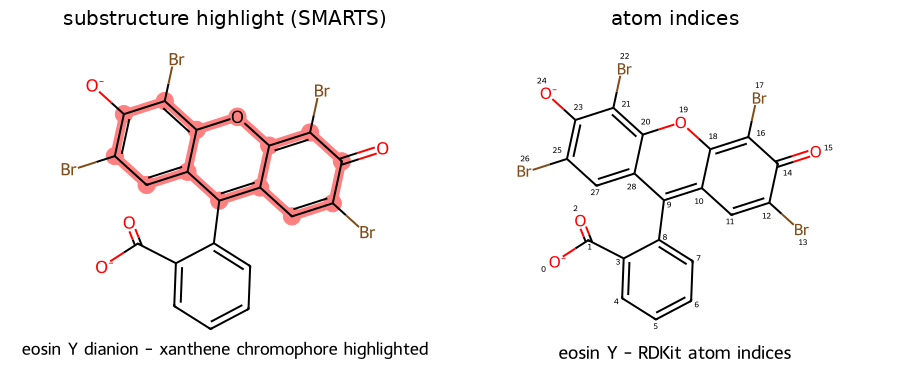
\includegraphics[width=0.8\linewidth]{eosinY_2d_tools.png}
\caption{Eosin~Y$^{2-}$: xanthene chromophore highlighted by SMARTS (left); RDKit atom indices
(right).}
\end{figure}

\begin{takeaway}
Look at the 2D picture of every molecule before any calculation. For Overleaf, export SVG
(\texttt{fmt="svg"}) rather than PNG, so it stays sharp at any size.
\end{takeaway}

%=============================================================================
\section{3D geometry: is the shape sensible?}

Coordinates come from RDKit: ETKDGv3 distance-geometry embedding followed by an MMFF94s
force-field minimisation. The final version embeds 8 conformers per molecule (30 when there are
more than three rotatable bonds) and keeps the lowest-energy one. A single random embedding is
fine for rigid dyes, but it can land in a poor local minimum for floppy ones.

\paragraph{Display styles each show something different}
\begin{itemize}
  \item \textbf{Ball-and-stick}: connectivity and angles. The default for checking a geometry.
  \item \textbf{Stick / line}: easier to read for large molecules such as TPP or 4CzIPN.
  \item \textbf{Space-filling}: atoms at van der Waals radii. Shows true size and crowding, and
  whether a molecule could lie flat on a surface or stack.
\end{itemize}

\begin{figure}[h]
\centering
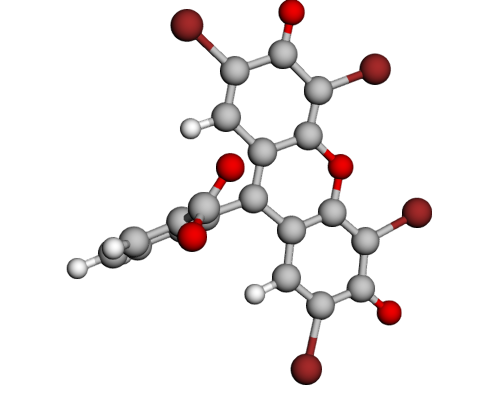
\includegraphics[width=0.38\linewidth]{eosinY_ballstick.png}\hspace{0.04\linewidth}
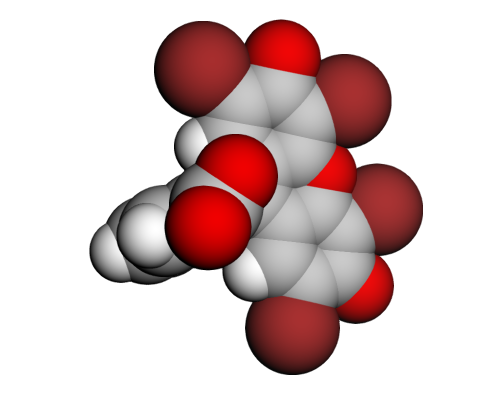
\includegraphics[width=0.38\linewidth]{eosinY_spacefill.png}
\caption{The same eosin~Y$^{2-}$ geometry in ball-and-stick (left) and space-filling (right).
Ball-and-stick shows the benzoate ring seen edge-on. Space-filling shows how much of the
molecule's volume the four bromines take up.}
\end{figure}

\paragraph{What the 3D pictures taught me about these catalysts}
Every one of these features is about \emph{twisting}, and twisting controls conjugation. Two
$\pi$ systems held perpendicular can't share electrons, so they behave as separate units.
\begin{itemize}
  \item \textbf{Eosin Y}: the benzoate ring is roughly perpendicular to the xanthene. I measured
  a ring--ring dihedral of \ang{98.6} in my MMFF geometry. That's why the benzoate barely
  affects the colour: it is electronically cut off from the chromophore.
  \item \textbf{TPP}: the four \emph{meso}-phenyls are twisted out of the porphyrin plane, so
  the absorbing $\pi$ system is essentially the porphyrin macrocycle alone.
  \item \textbf{4CzIPN}: the four carbazoles are twisted out of the plane of the
  dicyanobenzene. That decoupling separates donor from acceptor, which is the design principle
  behind its thermally activated delayed fluorescence (TADF) and photoredox behaviour.
  \item \textbf{Mes-Acr$^+$}: the mesityl ring is held orthogonal to the acridinium by its two
  ortho-methyl groups. Same idea: a donor and an acceptor in one molecule but electronically
  apart, which is why its excited state is so strongly oxidising.
  \item \textbf{Riboflavin}: the flexible ribityl tail can take many shapes. One conformer is
  only a sample, which is a limitation to state.
\end{itemize}

\begin{figure}[h]
\centering
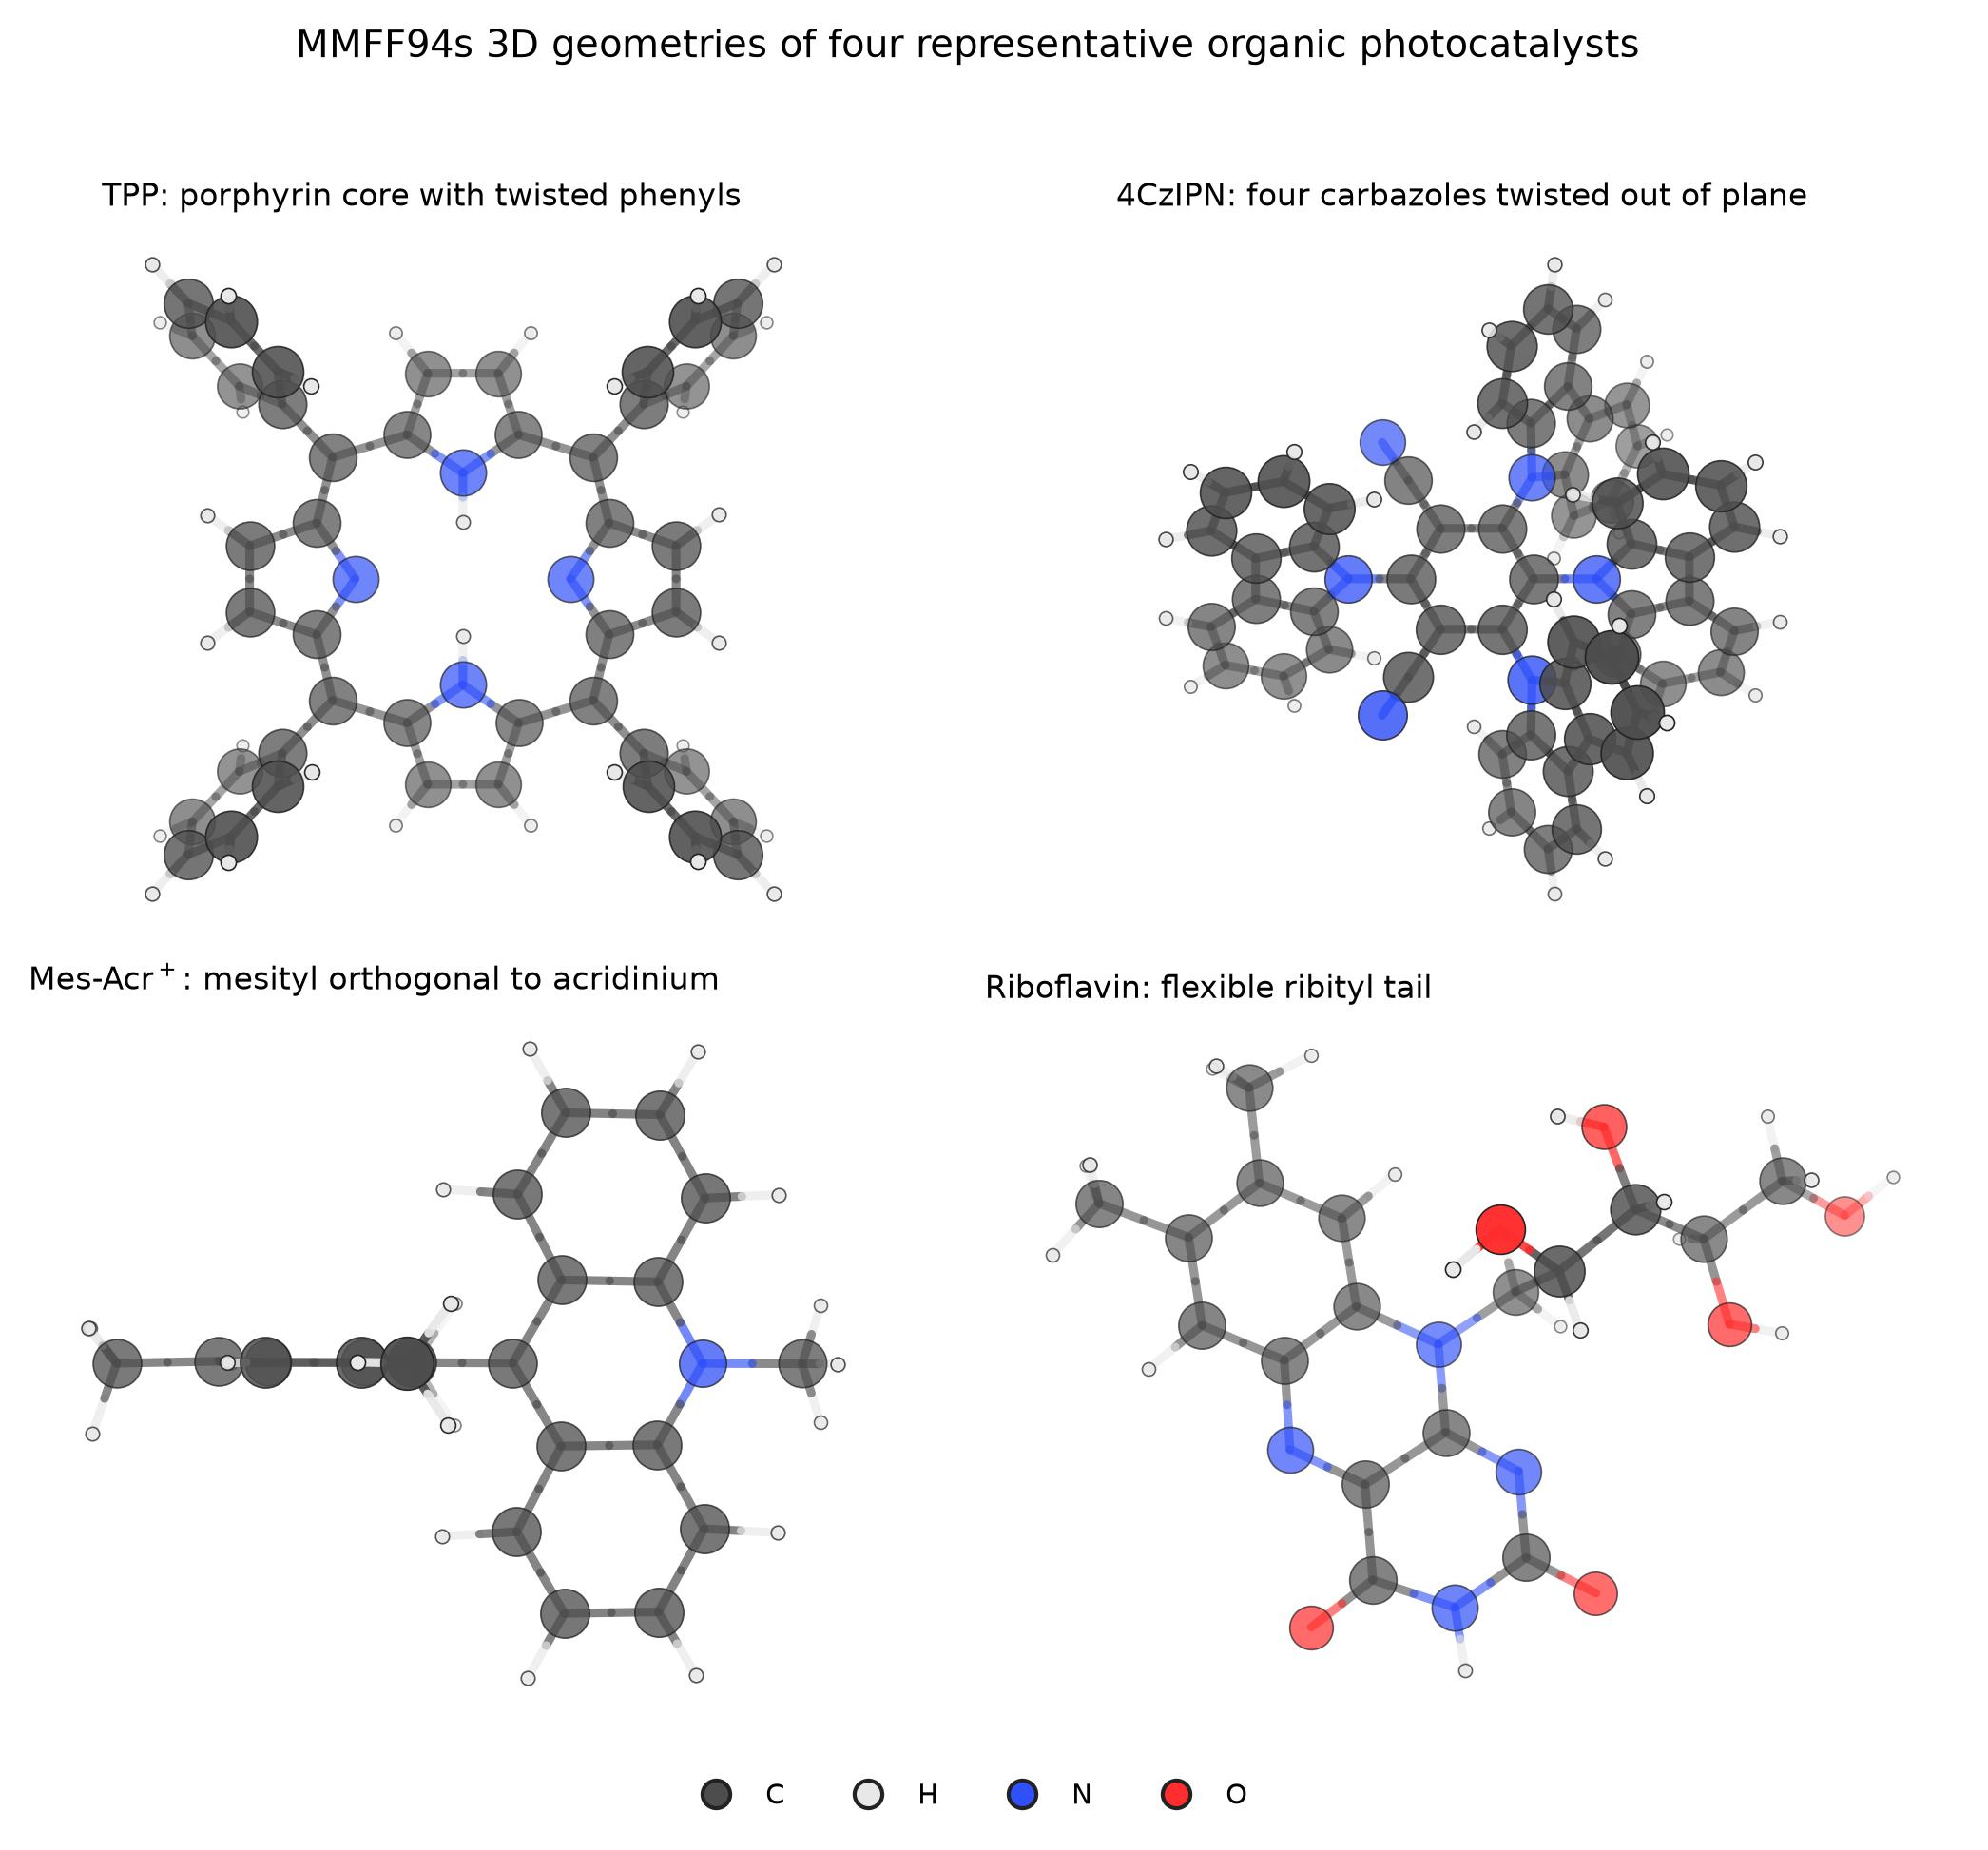
\includegraphics[width=0.85\linewidth]{structures_3d_montage.png}
\caption{MMFF94s geometries of four photocatalysts, each showing one structural motif.}
\end{figure}

\begin{takeaway}
Measure, don't eyeball. ``Looks perpendicular'' becomes a dihedral angle
(\texttt{rdMolTransforms.GetDihedralDeg}). ``Looks the same'' becomes an RMSD. A number goes in
the notes; an impression doesn't.
\end{takeaway}

%=============================================================================
\section{Overlays: how much did DFT change the structure?}

Overlaying the force-field start with the DFT result is the honest way to decide whether the
cheap geometry is good enough. Benzophenone was the instructive case:

\begin{figure}[h]
\centering
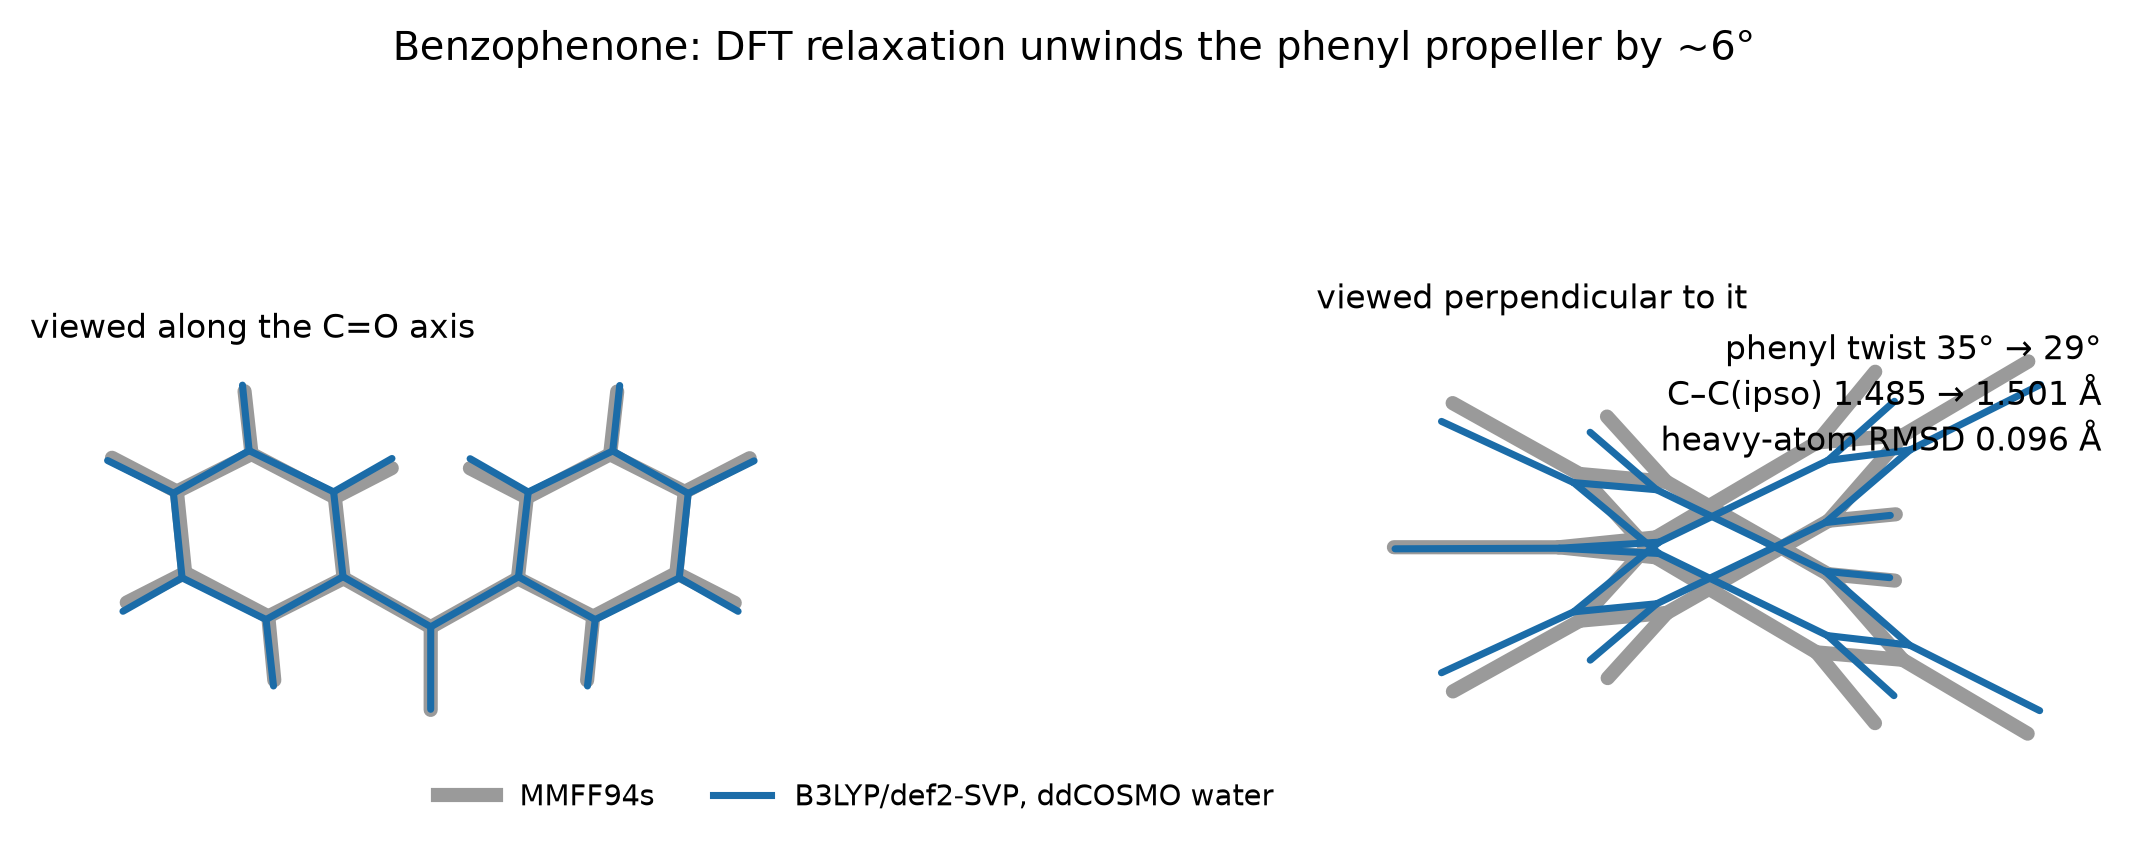
\includegraphics[width=0.95\linewidth]{geomopt_overlay_benzophenone.png}
\caption{MMFF94s (grey) vs B3LYP/def2-SVP in ddCOSMO water (blue). The right-hand view makes
the change in twist visible; the left-hand view hides it completely.}
\end{figure}

\begin{center}
\begin{tabular}{@{}lccc@{}}
\toprule
Molecule & RMSD$_\text{heavy}$ (\si{\angstrom}) & Cycles & $\Delta E$ (kcal/mol) \\
\midrule
anthraquinone (rigid) & 0.019 & 15 & $-1.42$ \\
thioxanthone (rigid) & 0.030 & 10 & $-1.88$ \\
benzophenone (2 rotatable rings) & 0.096 & 11 & $-1.27$ \\
\bottomrule
\end{tabular}
\end{center}

\noindent For benzophenone, DFT unwound the phenyl ``propeller'' from \ang{35} to \ang{29} and
lengthened the C--C$_\text{ipso}$ bond from 1.485 to \SI{1.501}{\angstrom}.

\begin{takeaway}
\begin{itemize}[leftmargin=*]
  \item The viewing angle can hide the difference. Always look along at least two
  perpendicular directions.
  \item MMFF is very good for rigid fused rings ($\le$\SI{0.03}{\angstrom}) but noticeably worse
  for torsions between rings. Errors concentrate exactly where conjugation is decided.
  \item So validating MMFF on three rigid molecules does \emph{not} justify using it for the
  floppy or charged ones (rhodamine~B, riboflavin, eosin~Y$^{2-}$). Those still need a DFT
  optimisation, or the limitation stated.
\end{itemize}
\end{takeaway}

%=============================================================================
\section{Orbitals: where are the electrons?}

\paragraph{How the picture is made.} PySCF evaluates an orbital on a 3D grid and writes a
\textbf{Gaussian cube file}. That's a plain-text format that py3Dmol, VESTA, VMD, Avogadro and
Jmol all read. An orbital has a sign, so it is drawn as two isosurfaces, $+\text{iso}$ and
$-\text{iso}$, in two colours.
\begin{itemize}
  \item Where the colour flips there is a \textbf{node}: a surface where the orbital is zero.
  \item The colours are arbitrary. Swapping blue and red gives the same orbital, since
  $\psi$ and $-\psi$ are physically identical.
  \item The \textbf{isovalue is a choice} (0.02--0.05~a.u.\ is conventional). Use the same
  value for every orbital you compare.
\end{itemize}

\begin{figure}[h]
\centering
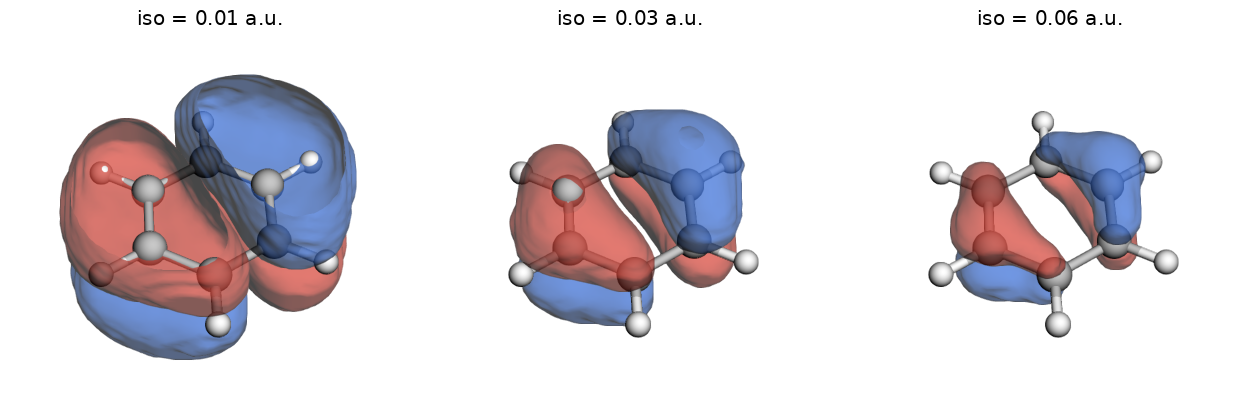
\includegraphics[width=0.95\linewidth]{benzene_isovalue_series.png}
\caption{The same benzene HOMO at three isovalues. The lobes shrink and swell, but the
\emph{nodes stay put}. The nodal pattern is the physics; the lobe size is a display choice.}
\end{figure}

\paragraph{Benzene: the textbook check.}
\begin{figure}[h]
\centering
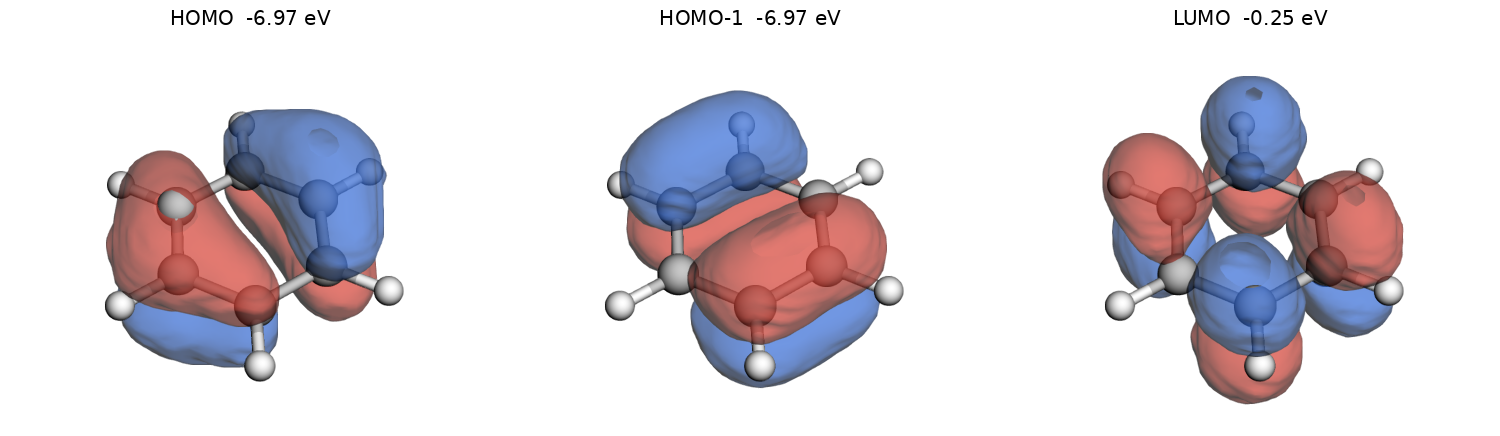
\includegraphics[width=0.95\linewidth]{benzene_frontier.png}
\caption{Benzene B3LYP/def2-SVP frontier orbitals, $\pm 0.03$~a.u.}
\end{figure}
\begin{itemize}
  \item HOMO and HOMO$-1$ have the same energy ($-6.97$~eV). They are a degenerate pair
  ($e_{1g}$ in $D_{6h}$), each with one nodal plane through the ring. The orientation the program
  prints is arbitrary, since any mixture of the two is equally valid. \textbf{Never interpret
  one member of a degenerate pair on its own.}
  \item The LUMO has two nodal planes. More nodes means higher energy: the particle-on-a-ring
  picture, seen directly.
\end{itemize}

\paragraph{Photocatalysts: local vs charge-transfer excitation.}
\begin{figure}[h]
\centering
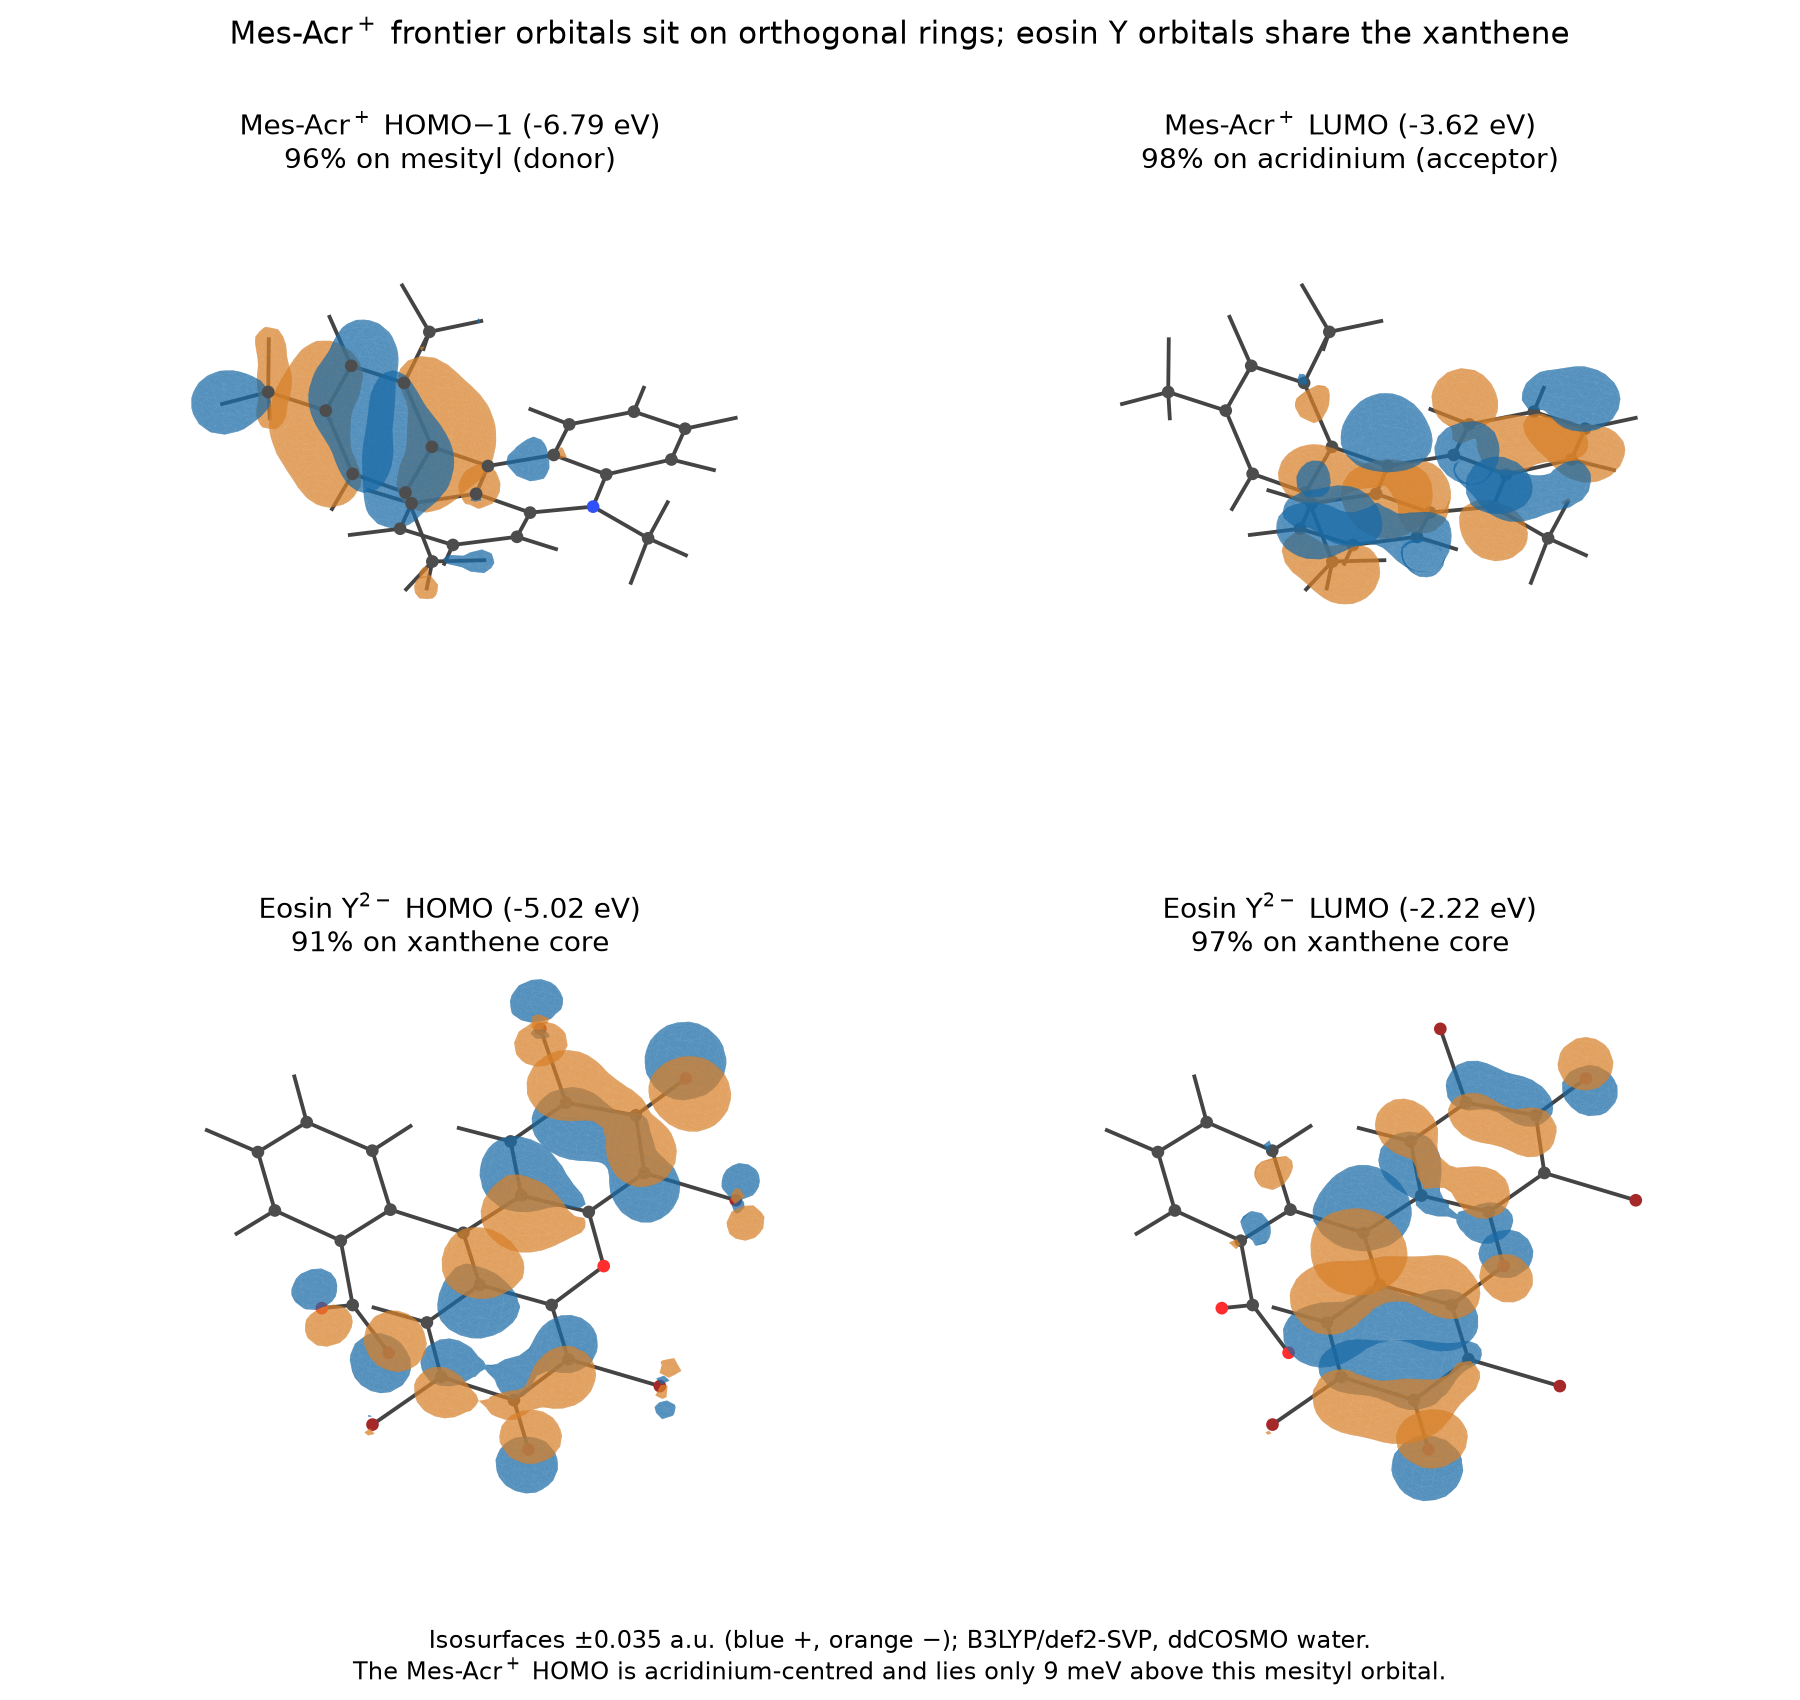
\includegraphics[width=0.78\linewidth]{frontier_orbitals_isosurfaces.png}
\caption{Mes-Acr$^+$ (top) and eosin~Y$^{2-}$ (bottom), B3LYP/def2-SVP in ddCOSMO water,
$\pm0.035$~a.u.}
\end{figure}

Pictures alone are not enough here, so each orbital was also split into fragment percentages
(Mulliken populations):

\begin{center}
\begin{tabular}{@{}llrl@{}}
\toprule
Molecule & Orbital & $E$ (eV) & Where it lives \\
\midrule
Eosin~Y$^{2-}$ & HOMO & $-5.02$ & 91\% xanthene core \\
               & LUMO & $-2.22$ & 97\% xanthene core \\
Mes-Acr$^+$    & HOMO$-2$ & $-6.80$ & $>$99\% mesityl \\
               & HOMO$-1$ & $-6.79$ & 96\% mesityl \\
               & HOMO     & $-6.79$ & 99\% acridinium \\
               & LUMO     & $-3.62$ & 98\% acridinium \\
\bottomrule
\end{tabular}
\end{center}

\begin{itemize}
  \item \textbf{Eosin Y}: HOMO and LUMO both sit on the xanthene, so the lowest excitation is a
  \emph{local} $\pi\to\pi^*$ excitation.
  \item \textbf{Mes-Acr$^+$}: the LUMO is on the acridinium acceptor, and mesityl donor orbitals
  sit just below the HOMO. Exciting from mesityl to acridinium moves charge between two
  orthogonal rings: a \emph{charge-transfer} state. This links directly back to the 3D
  picture in Section~2.
  \item The three top occupied orbitals of Mes-Acr$^+$ lie within 13~meV of each other, which
  is far below the accuracy of B3LYP. \textbf{Which one is ``the HOMO'' is not meaningful
  here}, so look at the set, not the label.
\end{itemize}

\begin{takeaway}
Pair every orbital picture with a number: the fragment percentage, the energy, and how close it
is to its neighbours. Mulliken percentages depend on the basis set, so treat them as
fragment-level indicators (91\% vs 10\%), not precise values. For charge-transfer molecules
(Mes-Acr$^+$, 4CzIPN), B3LYP underestimates the excitation energy; use a range-separated
functional (CAM-B3LYP, $\omega$B97X-D) for TDDFT.
\end{takeaway}

%=============================================================================
\section{Energy-level diagrams: the picture that misleads most easily}

Plotting HOMO/LUMO for all 16 molecules side by side is a good way to see trends. The
Kohn--Sham gap tracks the lowest experimental absorption band well ($r = 0.90$, MAE 0.45~eV,
$n=16$). The biggest outlier, benzophenone (+1.37~eV), is explained by its weak first band
being n$\to\pi^*$, not $\pi\to\pi^*$.

\begin{pitfall}
Drawing the H$^+$/H$_2$ and O$_2$/H$_2$O levels across Kohn--Sham orbital energies invites the
reader to read off redox driving forces, and the numbers don't support that. As I found with
benzene, $-\varepsilon_\text{HOMO}$ underestimates the ionisation energy by about 2~eV for B3LYP,
and the HOMO--LUMO gap is neither the fundamental nor the optical gap. A good correlation with
absorption shows the \emph{trend} is right, not that the absolute positions are. For redox
potentials, compute energy differences between charge states in solvent ($\Delta$SCF); for
absorption, use TDDFT.
\end{pitfall}

%=============================================================================
\section{Practical notes on tools}

\begin{itemize}
  \item \textbf{RDKit}: identifiers, 2D drawing, conformers, xyz export, dihedrals and RMSD.
  \item \textbf{py3Dmol}: the quickest interactive viewer in Jupyter, and it writes standalone
  HTML I can send to my PI. It has no headless PNG export, so static figures need a workaround.
  I used a headless browser (Playwright + Chromium); the Claude Science run used marching
  cubes in matplotlib. matplotlib only approximates which surface is in front, so treat those
  as schematic.
  \item \textbf{VESTA / VMD}: what to use for figures with proper lighting and depth. VESTA also
  handles crystal structures, which I'll need in Week~2.
  \item \textbf{Cube files} are 3--5~MB each. Keep them out of git (\texttt{*.cube} in
  \texttt{.gitignore}) and regenerate them, which takes seconds once the SCF is done.
\end{itemize}

\begin{howto}
\raggedright
\begin{itemize}[leftmargin=*]
  \item 2D: \texttt{viz.draw\_2d(smiles, highlight\_smarts=..., atom\_indices=True)}
  \item 3D: \texttt{viz.view\_xyz(xyz, "ballstick" | "sphere" | "stick")}
  \item Overlay: \texttt{viz.overlay\_xyz(xyz\_mmff, xyz\_dft)}
  \item Orbital: \texttt{cubegen.orbital(mol, "x.cube", mf.mo\_coeff[:, i])}, then
  \texttt{viz.view\_orbital("x.cube", iso=0.03)}
  \item Everything is in \texttt{molecules/visualize.ipynb} (or the self-contained
  \texttt{visualize\_molecules.ipynb}).
\end{itemize}
\end{howto}

%=============================================================================
\section{Checklist I'll reuse}

\begin{enumerate}
  \item 2D picture of every input: right atoms, right charge, right protonation state?
  \item 3D picture: rings flat where they should be, twisted where sterics demand it? Measure
  the key dihedrals.
  \item Overlay MMFF vs DFT from two viewing directions; record heavy-atom RMSD.
  \item Orbitals: same isovalue for everything; check for degenerate or near-degenerate partners
  before naming ``the HOMO''.
  \item Put a number next to every picture (energy, \% localisation, dihedral, RMSD).
  \item Never read redox potentials or absorption energies off Kohn--Sham orbital energies.
  \item Label every figure with its level of theory (functional/basis/solvent). These runs used
  B3LYP/def2-SVP in ddCOSMO water,
  with \emph{no} D3 dispersion.
\end{enumerate}

\end{document}
